
\documentclass[twocolumn,12pt]{article}
\usepackage[left=1.5cm, right=1.5cm, bottom=2cm, top=2cm]{geometry}
\usepackage[utf8]{inputenc}
\usepackage{mathptmx}
\usepackage{fancyhdr}
\usepackage{latexsym}
\usepackage{booktabs,chemformula}
\usepackage{multirow,array}
\usepackage{multicol}
\usepackage{natbib}
\usepackage{graphicx}
\usepackage{colortbl}
\usepackage{indentfirst}
\usepackage{amsmath}
\usepackage[english]{babel}
\usepackage[capposition=top]{floatrow}

\usepackage[compact]{titlesec}
\titlespacing{\section}{1pt}{2ex}{2ex}
\titlespacing{\subsection}{1pt}{1ex}{1ex}

\definecolor{indigo(dye)}{rgb}{0.0, 0.25, 0.42}
\definecolor{lightgreen}{rgb}{0.56, 0.93, 0.56}
\definecolor{lightpink}{rgb}{1.0, 0.71, 0.76}
\definecolor{lightyellow}{rgb}{0.98, 0.98, 0.82}

\setlength{\parindent}{20pt}
\setlength{\parskip}{\baselineskip}

\let\oldheadrule\headrule% Copy \headrule into \oldheadrule
\renewcommand{\headrule}{\color{indigo(dye)}\oldheadrule}
\pagestyle{fancy}
\fancyhf{}
\rhead{\thepage}
\lhead{\textcolor{indigo(dye)}{US Unemployment Rate VS. Median House Sale Price in the US.}}

\usepackage{titling}
\setlength{\droptitle}{-1cm}

\begin{document}

\title{\textbf{\textcolor{indigo(dye)}{Relationship between the US Unemployment Rate and Median House Sale Price in the US.}}}
\author{\textbf{\textcolor{indigo(dye)}{Hanlu Xia}}}
\date{\textbf{\textcolor{indigo(dye)}{Dec 1, 2024}}}
\maketitle

\section*{\textcolor{indigo(dye)}{Introduction}}

Unemployment is an important indicators used to explain US economy performance, and it is proved to be highly correlated to recession. On the other hand, Housing market is always involved either directly or indirectly in US recession, especially in 2008.

This analysis wants to explore whether housing price can be used an a predictor to US recession (using umeployment rate to represent the recession cycle). They are very likely to have a negative correlation as housing market usually goes down when unemployment goes up. It's also very likely there would be lagging effects between the two, as housing market usually starts to go down before umemployment starts to go up. If there are measurable lags, how many months would that be?

\section*{\textcolor{indigo(dye)}{Exploratory Analysis}}
This shows the Time Series Plot of Raw data, and the stationary analysis of raw data and their first difference.

\begin{figure*}[ht]
\centering
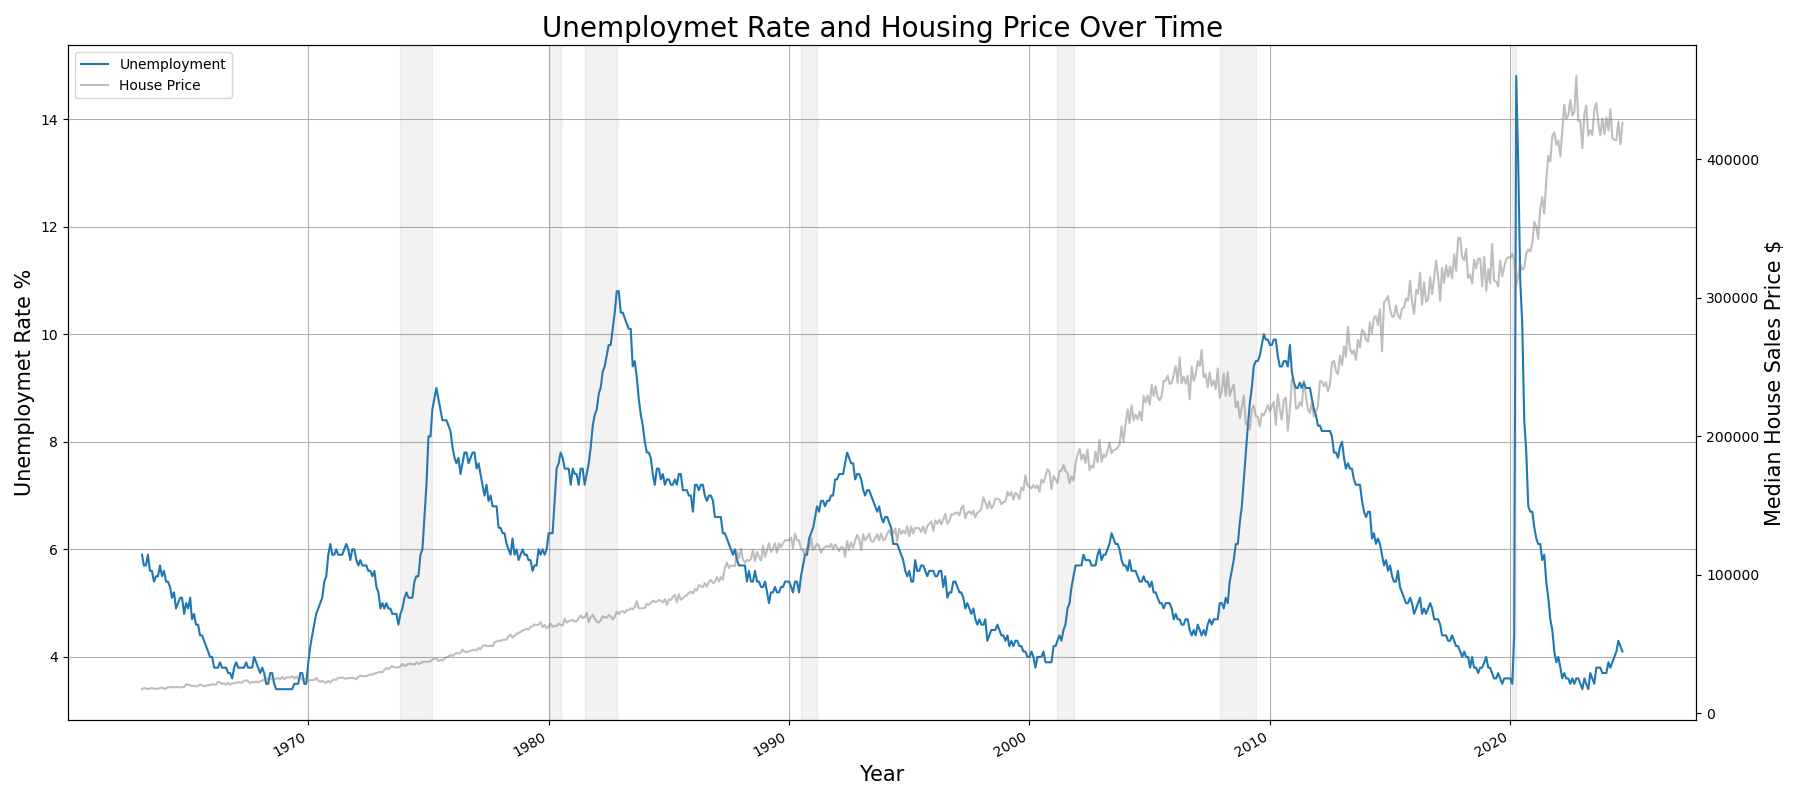
\includegraphics[width=1\textwidth]{C:/Users/siaha/PycharmProjects/Unemployment_House/Analytics_Output/timeseries1.png}
\caption{Unemployment Vs. House Price}
\end{figure*}

The following table represents the stationary analysis:


\begin{table}[H]
\scalebox{0.8}{
\begin{tabular}{@{} l*{3}{>{}c<{}} @{}}
\toprule
Description & P-Value & Result & \\
\midrule
Unemployment Rate & 0.017 & stationary  \\
Median Housing Price Over Time & 0.997 & non-stationary  \\
First diff of housing Price & 0.0 & stationary  \\
Return of housing Price & 0.0 & stationary  \\

\bottomrule
\end{tabular}}
\caption{Stationary Analysis}
\end{table}

\subsection*{\textcolor{indigo(dye)}{Correlation Analysis of Raw data and First Difference}}

Some text to fill here; Some text to fill here; Some text to fill here; Some text to fill here; Some text to fill here; 

\begin{figure}[H]
\centering
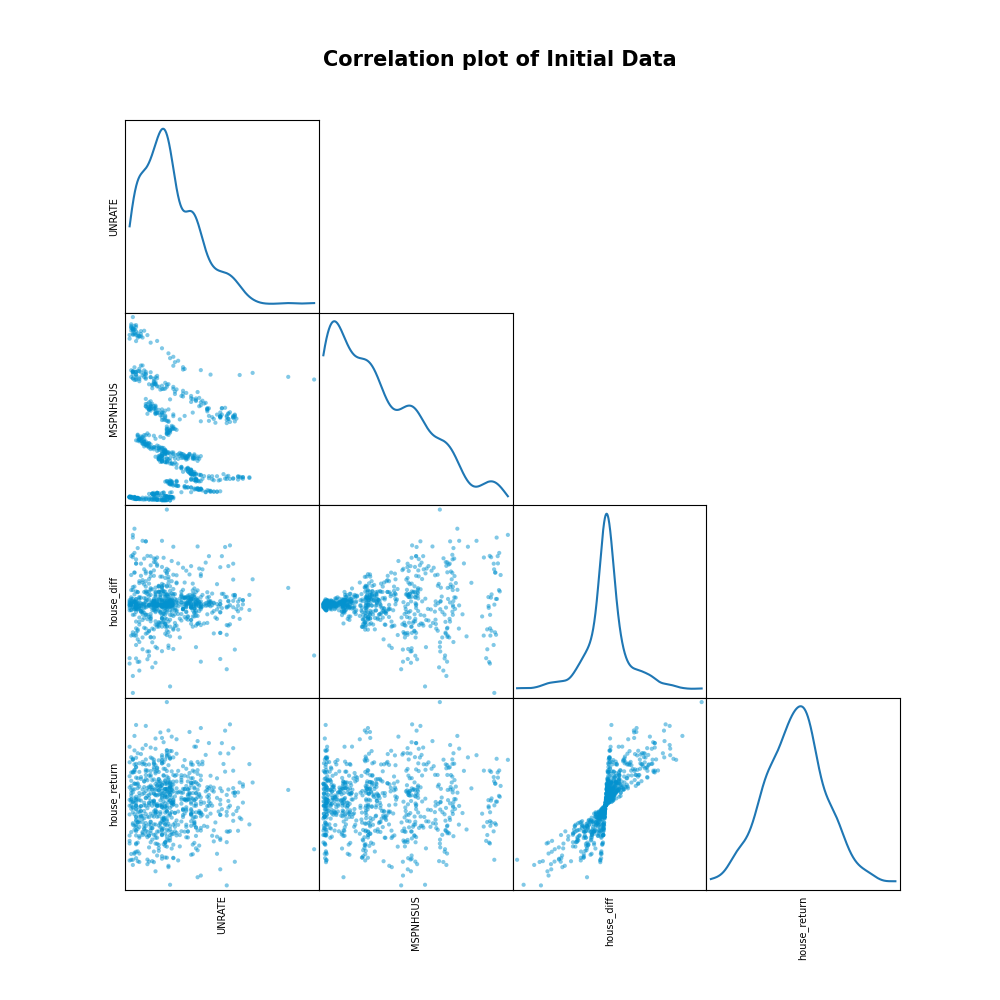
\includegraphics[width=1\textwidth]{C:/Users/siaha/PycharmProjects/Unemployment_House/Analytics_Output/correlationplot1.png}
\caption{Correlation Plot of Raw data and First Difference }
\end{figure}

\begin{figure}[H]
\centering
\scalebox{1}{
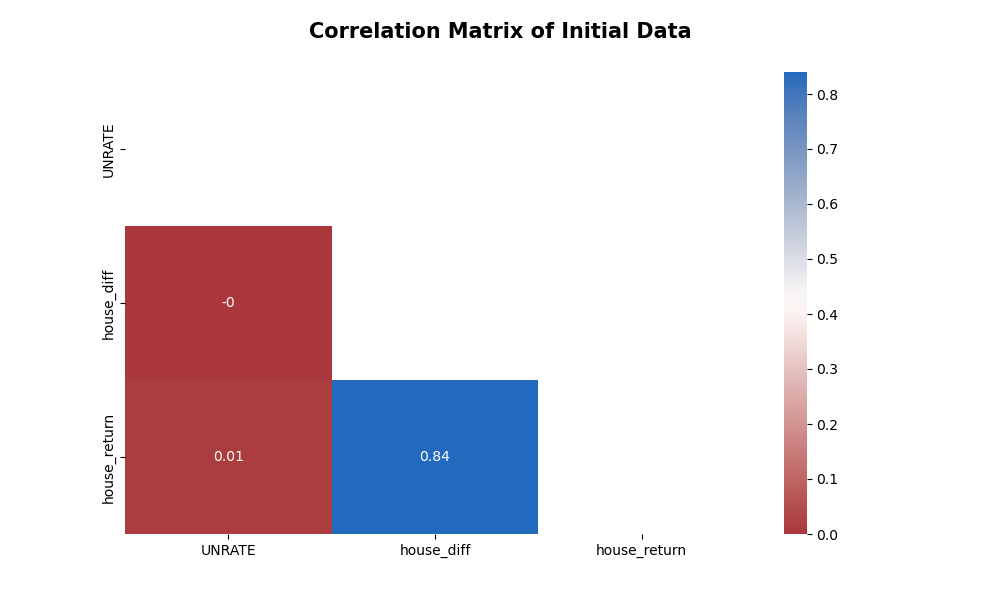
\includegraphics[width=1\textwidth]{C:/Users/siaha/PycharmProjects/Unemployment_House/Analytics_Output/corrmatrix1.png}}
\caption{Correlation Matrix of Raw data and First Difference}
\end{figure}

\section*{\textcolor{indigo(dye)}{Regression Analysis}}

Some text to fill here; Some text to fill here; Some text to fill here; Some text to fill here; Some text to fill here; 

\begin{table}[H]
\scalebox{1}{
\begin{tabular}{@{} l*{3}{>{}c<{}} @{}}
\toprule
Total Lag & R2 & Change in R2 & \\
\midrule
1.0 & 0.017 & 0.017  \\
2.0 & 0.034 & 0.017  \\
3.0 & 0.056 & 0.022  \\
4.0 & 0.077 & 0.021  \\
5.0 & 0.1 & 0.022  \\
6.0 & 0.12 & 0.02  \\
7.0 & 0.136 & 0.016  \\
8.0 & 0.149 & 0.013  \\
9.0 & 0.16 & 0.011  \\
10.0 & 0.171 & 0.01  \\
11.0 & 0.176 & 0.005  \\
12.0 & 0.181 & 0.006  \\
13.0 & 0.186 & 0.005  \\
14.0 & 0.191 & 0.005  \\
15.0 & 0.194 & 0.003  \\
16.0 & 0.197 & 0.003  \\
17.0 & 0.199 & 0.003  \\
18.0 & 0.202 & 0.002  \\
19.0 & 0.206 & 0.004  \\
20.0 & 0.21 & 0.004  \\
21.0 & 0.215 & 0.005  \\
22.0 & 0.22 & 0.006  \\
23.0 & 0.227 & 0.007  \\
24.0 & 0.233 & 0.006  \\

\bottomrule
\end{tabular}}
\caption{Regression and Lags}
\label{market_crash}
\end{table}

\begin{figure}[H]
\centering
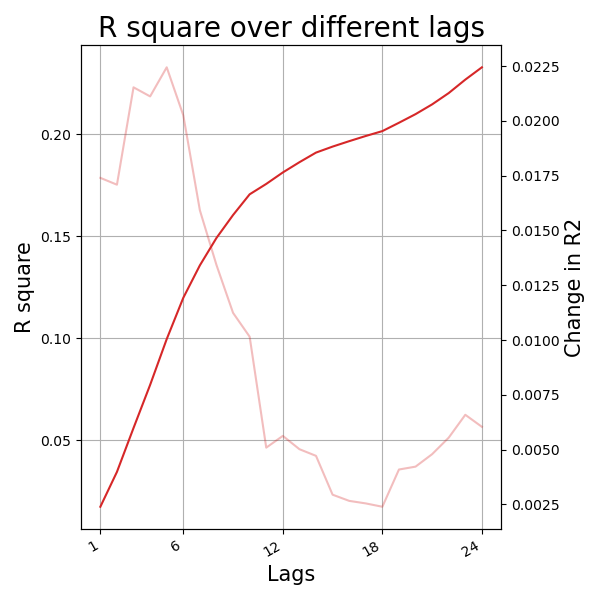
\includegraphics[width=1\textwidth]{C:/Users/siaha/PycharmProjects/Unemployment_House/Analytics_Output/regression_result.png}
\caption{Change in R2 Over Lags}
\end{figure}


\section*{\textcolor{indigo(dye)}{Correlation with Optimized Lag}}

Some text to fill here; Some text to fill here; Some text to fill here; Some text to fill here; Some text to fill here; 

\begin{figure*}[h!]
\centering
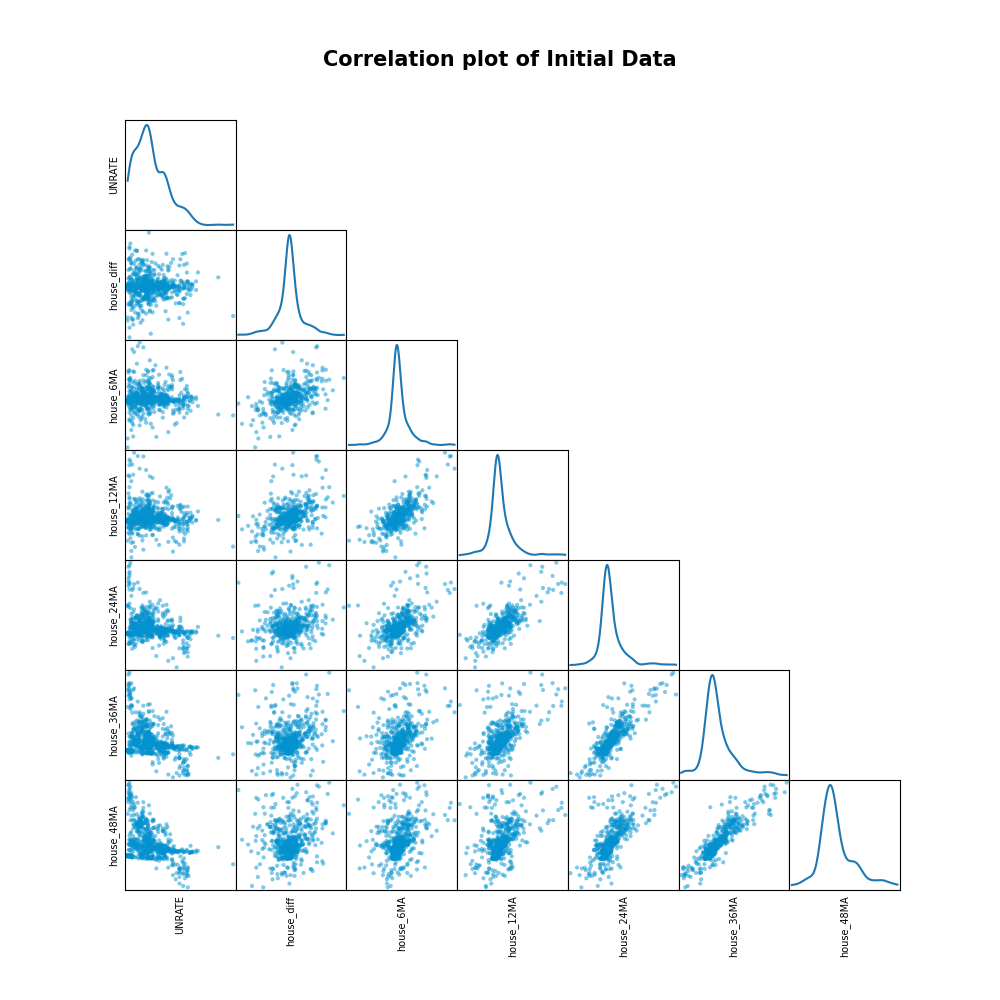
\includegraphics[width=1\textwidth]{C:/Users/siaha/PycharmProjects/Unemployment_House/Analytics_Output/correlationplot2.png}
\caption{Correlation Plot After Lag}
\end{figure*}

\begin{figure*}[h!]
\centering
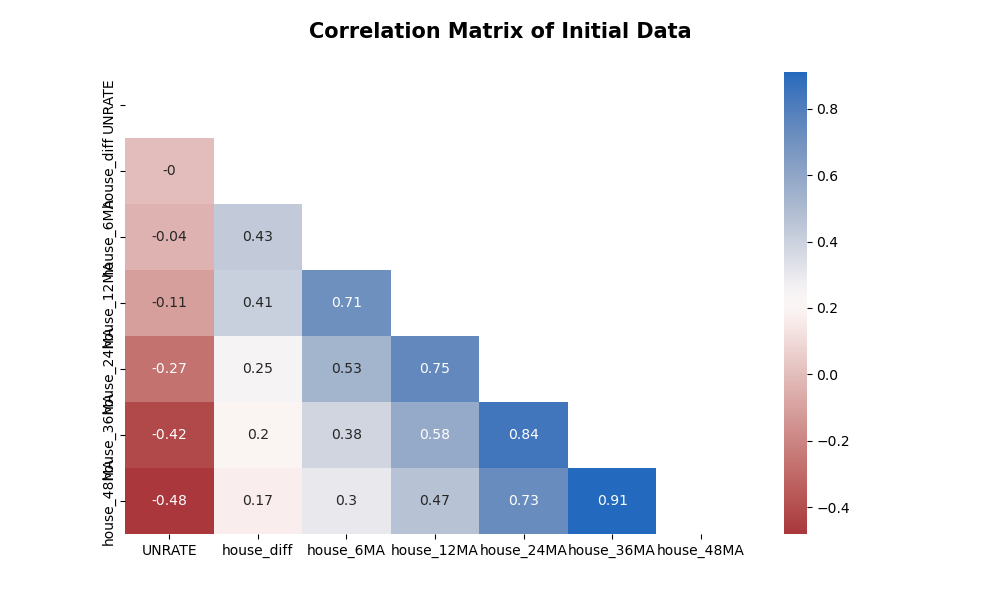
\includegraphics[width=1\textwidth]{C:/Users/siaha/PycharmProjects/Unemployment_House/Analytics_Output/corrmatrix2.png}
\caption{Correlation Matrix After Lag}
\end{figure*}

\section*{\textcolor{indigo(dye)}{Conclusion}}
Based on analysis above, it is statistically confident enough to say that housing price is a predictor of the unemployment rate with 11 month lags.

\begin{figure*}[h!]
\centering
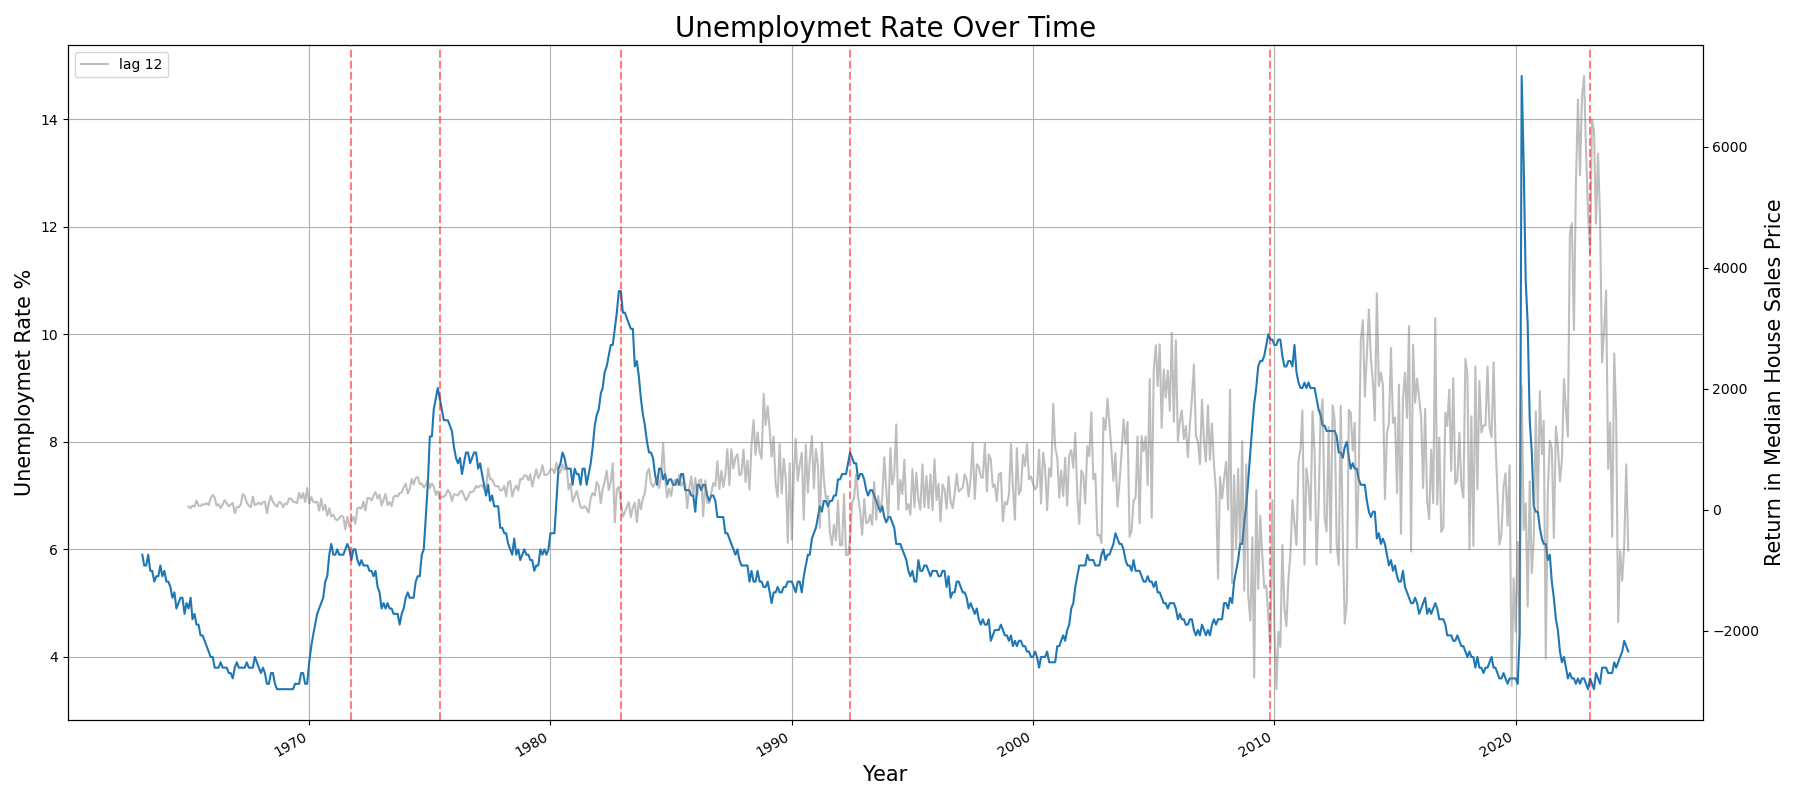
\includegraphics[width=1\textwidth]{C:/Users/siaha/PycharmProjects/Unemployment_House/Analytics_Output/timeseries2.png}
\caption{Unemployment Rate Vs. House Price with 11 lags}
\end{figure*}


\end{document}
    